\chapter{Analyse}\label{ch:analyse}

Nu hvor kravene for systemet er sat, kan analyse og design aktiviteten under Unified Process påbegyndes. Under analysen er SSD-diagrammet blevet konstrueret, samt operationskontrakt. Derefter kan systemet designes. 

\section{Systemsekvensdiagram}
Systensekvensdiagrammet\cite{Larman2004} adresserer, hvordan brugeren og systemet kommunikerer frem og tilbage. Dette SSD-diagram er lavet ud fra Fully Dressed Use Case, automatisk lagerstyring.

\begin{figure}[H]
    \centering
    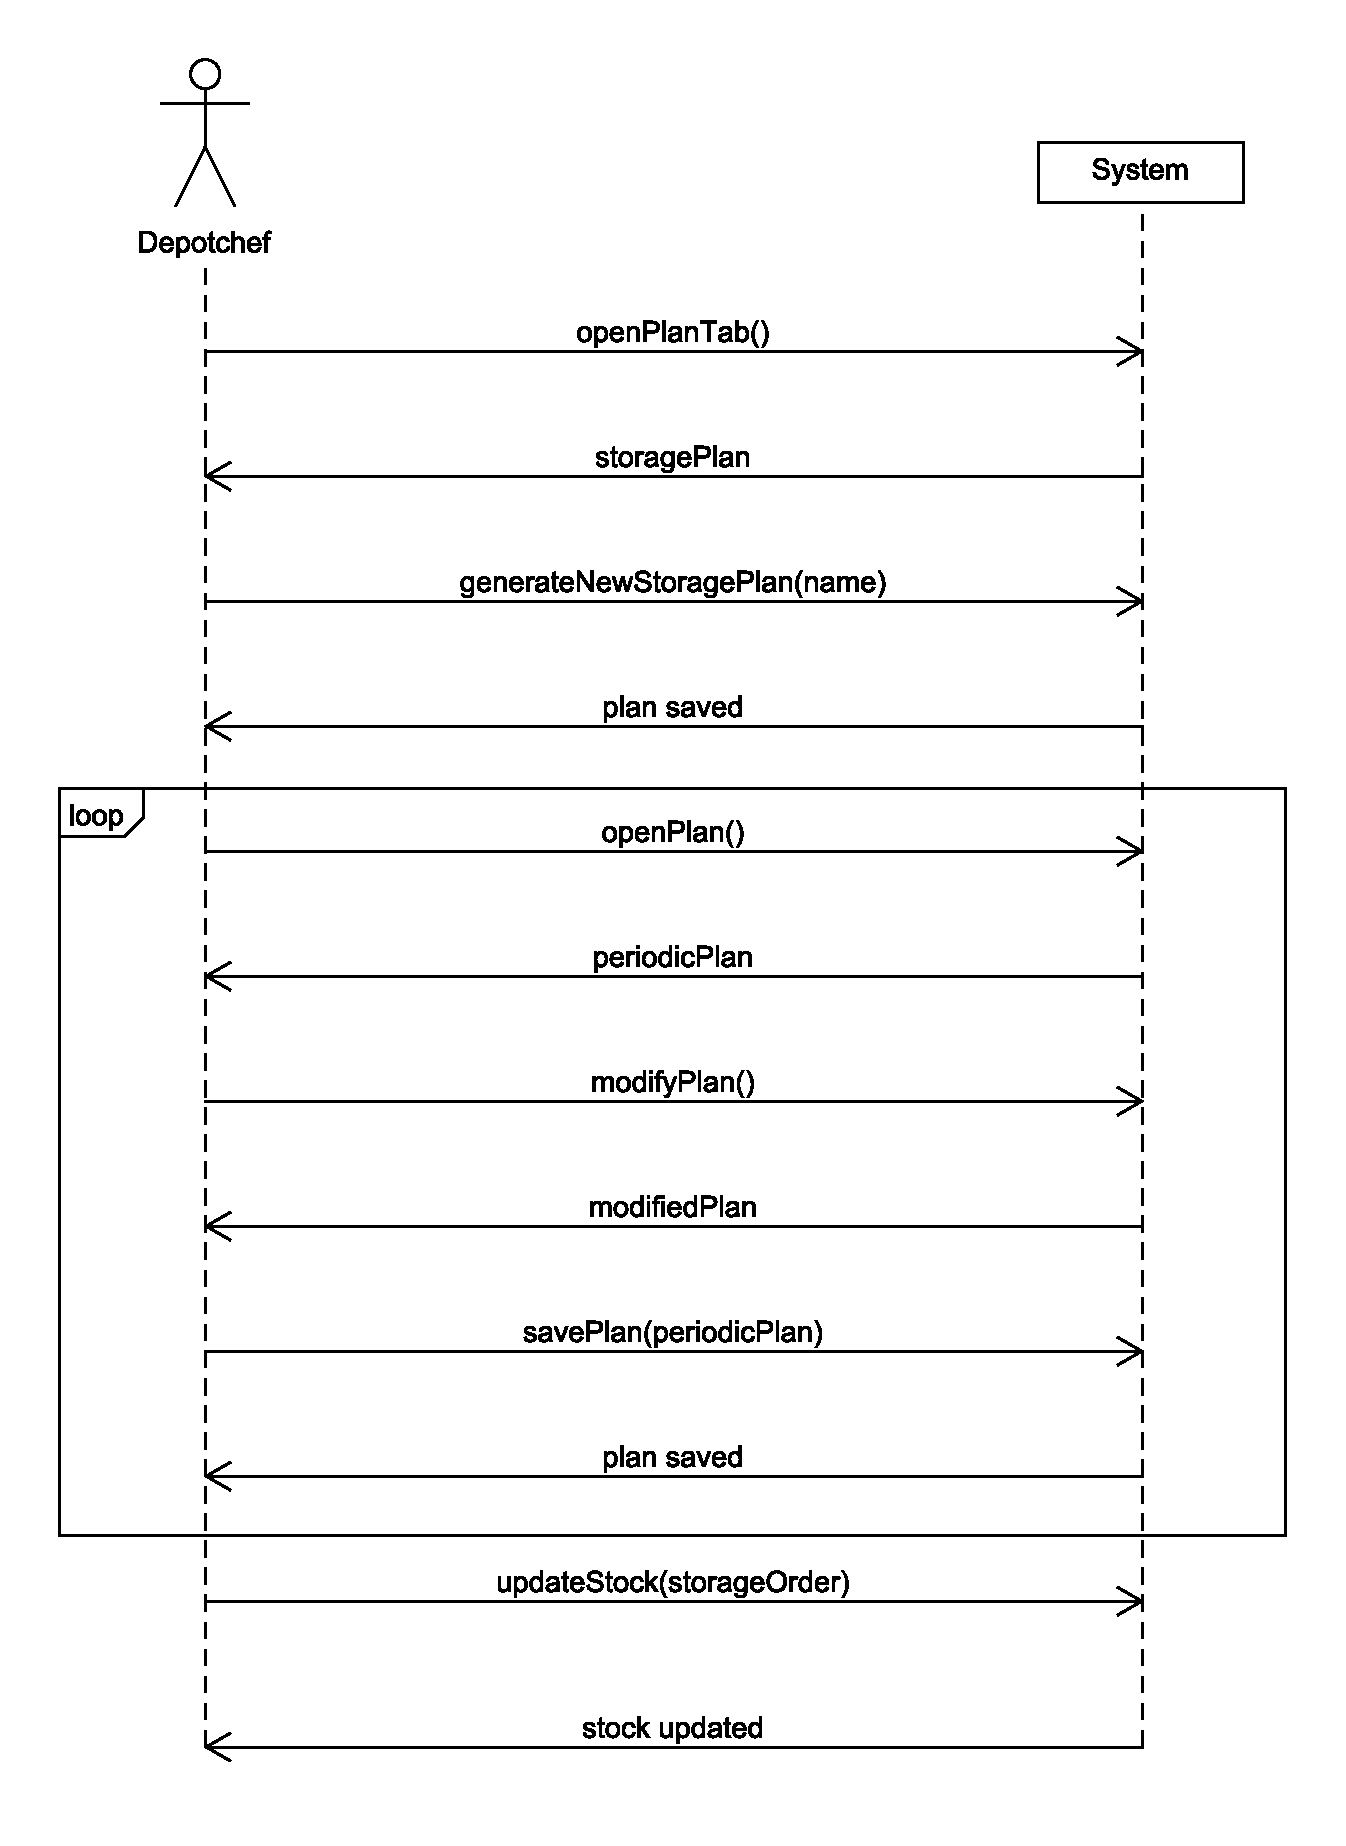
\includegraphics[width=100mm]{figures/analyse/SSD.eps}
    \caption{Systemsekvensdiagram}
    \label{fig:ssd}
\end{figure}

Her ses det, at depotchef Niels Thomas er den eneste, som benytter systemet. Som det første åbner Niels Thomas den nuværede plan for lageret, hvorefter vil systemet give den nuværende lager plan. 

Når den er åbnet kan Niels Thomas generere en ny lager plan \verb|generateNewStoragePlan(name)|, samt navngive planen. Denne funktion generer en plan, baseret på salgsdata, produkters popularitet og kommende udsalg. Når planen er genereret, vil den blive ved med at oprette storageOrders, baseret på den oprettede plan. 
Såfremt planen har brug for ændring, skal der genereres en ny plan. Det er muligt at åbne den og foretage ændringer i planen. Et eksempel kunne være, at man ville have 20 isbåde istedet for 10. Herefter gemmes planen og storageOrders oprettes automatisk på ubestemt tid. 
Så snart de varer bestilt med en StorageOrder er ankommet til varehuset, opdateres lageret ud fra hvilke produkter der blev bestilt.

\section{Operationskontrakt}
Ud fra SSD diagrammet og Fully Dressed Use Casen kan der udvikles en Operationskontrakt\cite{Larman2004}. Operationskontrakten beskriver i flere detaljer hvad der sker af ændringer i programmet under hvert trin i use casen. Noget som ikke fremkommer tydeligt under disse trin er, at så snart en StoragePlan er genereret vil denne indeholde en masse PeriodicPlans. Disse PeriodicPlan er tænkt som værende f.eks. en ugeplan, og der vil derfor være mange PeriodicPlans i en StoragePlan. Når de er oprettet, vil PeriodicPlan oprette en StorageOrder, som er en varebestilling. Såfremt perioden er for en uge, vil der hver uge tages en ny PeriodicPlan som opretter en ny StorageOrder. Dette fortsætter indtil der ikke er flere PeriodicPlans eller starter forfra ved at generere en ny StoragePlan.

\begin{center}
    \begin{longtable}{ |p{360pt}| }
        \hline
        \textbf{Operationskontrakt}
        \\
        \noindent\fbox{%
            \parbox{4.88in}{%
                \textbf{Operation:} openPlanTab() \\ Åbner planfanen i programmet
                
            }%
        }
        \\
        \noindent\fbox{%
            \parbox{4.88in}{%
                \textbf{Operation:} generateNewStoragePlan(name) \\ 
                Use Case: Bestil Varer \\

                Præ-betingelser: en instans af productMap eksisterer \\

                Post-betingelser: \\
                - sp.name blev sat til name \\
                - En instans af PeriodicPlan blev oprettet \\
                - pp.period blev sat til period \\
                - en instans af sOrder blev oprettet \\
                - pp blev associeret med product og sOrder \\
                - p blev associeret med supplier og productLine \\
                - sOrder blev associeret med supplier og productLine 
            }%
        }
        \\
        \noindent\fbox{%
            \parbox{4.88in}{%
                \textbf{Operation:} openPlan() \\
                Den generede plan åbnes i planfanen i programmet
            }%
        }
        \\
        \noindent\fbox{%
            \parbox{4.88in}{%
                \textbf{Operation:} savePlan(periodicPlan) \\
                Use Case: CRUD StoragePlan \\
                Præ-betingelser: En instans af StoragePlan eksisterer \\
                Post-betingelser: \\
                - De nye periodicPlan instanser gemmes i periodicPlans
            }%
        }
        \\
        \noindent\fbox{%
            \parbox{4.88in}{%
                \textbf{Operation:} updateStock(storageOrder) \\
                Use Case: Modtag Varer \\
                Præ-betingelser: Produkterne bestilt fra en storageOrder er ankommet til depotet. \\
                Post-betingelser: \\
                - sOrder.sentDate er blevet sat til sentDate \\
                - sOrder.trackingId er blevet sat til trackingId \\
                - productLine.amount er blevet opdateret
            }%
        }
        \\
        \hline
    \end{longtable}
\end{center}

Ud fra operationskontrakten og SSD kan der nu laves interaktionsdiagrammer og herefter designklassediagrammet, som vil være sidste blik for detaljer i design af systemet før det kan kodes.

